% Exercise ID: MAT_A12OTIMI_PROB_RAM_002
% Module: Módulo A12 - Otimização | Concept: Problemas Simples de Otimização
% Type: problemas_de_rampas | Difficulty: 2/5
% Tags: trigonometria, rampas, acessibilidade, angulo
% Author: Professor | Date: 2025-11-25

\exercicio{
Um edifício precisa de uma rampa de acesso que suba 50 cm de altura. O projetista quer que a inclinação da rampa seja exatamente de 4° (dentro das normas de acessibilidade).

\begin{center}
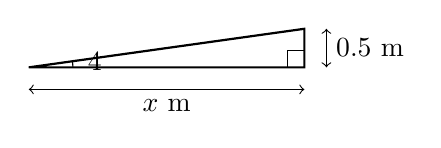
\begin{tikzpicture}[scale=0.7]
    \draw[thick] (0,0) -- (5,0) -- (5,0.7) -- cycle;
    \draw (4.7,0) rectangle (5,0.3);
    \draw[<->] (0,-0.4) -- (5,-0.4) node[midway,below] {$x$ m};
    \draw[<->] (5.4,0) -- (5.4,0.7) node[midway,right] {0.5 m};
    \draw (0.8,0) arc (0:8:0.8) node[right,xshift=2pt] {$4°$};
\end{tikzpicture}
\end{center}
}

\subexercicio{Qual razão trigonométrica relaciona a altura com o comprimento horizontal da rampa?}

\subexercicio{Sabendo que $\tan(4°) \approx 0.07$, calcula o comprimento horizontal $x$ necessário.}

\subexercicio{Qual seria o comprimento total da rampa (hipotenusa)? Usa o Teorema de Pitágoras.}

\subexercicio{Se o espaço disponível é de apenas 6 metros horizontais, a rampa pode ser construída com inclinação de 4°? Justifica.}
